\documentclass[journal=jmcmar,manuscript=article]{achemso}


%%%%%%%%%%%%%%%%%%%%%%%%%%%%%%%%%%%%%%%%%%%%%%%%%%%%%%%%%%%%%%%%%%%%%
%% Place any additional packages needed here.  Only include packages
%% which are essential, to avoid problems later. Do NOT use any
%% packages which require e-TeX (for example etoolbox): the e-TeX
%% extensions are not currently available on the ACS conversion
%% servers.
%%%%%%%%%%%%%%%%%%%%%%%%%%%%%%%%%%%%%%%%%%%%%%%%%%%%%%%%%%%%%%%%%%%%%
\usepackage[version=3]{mhchem} % Formula subscripts using \ce{}
\usepackage{subcaption}
\usepackage{array}
\usepackage{url}
\usepackage{xr}
%\usepackage{xr-hyper}
\usepackage{hyperref}
\usepackage{multirow}
\usepackage{listings}
\usepackage[finalizecache,cachedir=.]{minted}
\usepackage[flushleft]{threeparttable}
%\captionsetup[figure]{font=small,labelfont=small}

\lstset{
breaklines=true,
breakatwhitespace=true,
captionpos=b,
frame=single
}


\makeatletter
\newcommand*{\addFileDependency}[1]{% argument=file name and extension
  \typeout{(#1)}
  \@addtofilelist{#1}
  \IfFileExists{#1}{}{\typeout{No file #1.}}
}
\setlength\acs@tocentry@height{8.25cm}
\setlength\acs@tocentry@width{4.45cm}
\makeatother
\newcommand*{\myexternaldocument}[1]{%
    \externaldocument{#1}%
    \addFileDependency{#1.tex}%
    \addFileDependency{#1.aux}%
}

\myexternaldocument{supplement}
\newcommand*\mycommand[1]{\texttt{\emph{#1}}}


\title{SolTranNet -- A ML tool for fast aqueous solubility prediction.}
\keywords{deep learning, machine learning, molecular property prediction, solubility, tool}
\author{Paul G. Francoeur}
\author{David R. Koes}
\email{dkoes@pitt.edu}
\affiliation[Pitt]{Department of Computational and Systems Biology, University of Pittsburgh, Pittsburgh, PA 15260}

\begin{document}
%%%%%%%%%%%%%%%%%%%%%%%%%%%%%%%%%%%%%%%%%%%%%%%%%%%%%%%%%%%%%%%%%%%%%
%% The abstract environment will automatically gobble the contents
%% if an abstract is not used by the target journal.
%%%%%%%%%%%%%%%%%%%%%%%%%%%%%%%%%%%%%%%%%%%%%%%%%%%%%%%%%%%%%%%%%%%%%
\begin{abstract}
While accurate prediction of aqueous solubility remains a challenge in drug discovery, machine learning (ML) approaches have become increasingly popular to predict such values.
For instance, in the Second Challenge to Predict Aqueous Solubility contest, all participating groups utilized machine learning methods in their submission.
We present SolTranNet, a molecule attention transformer model to predict aqueous solubility from a molecule's SMILES representation.
Atypically, we demonstrate that larger models do not perform better at this task, with the final version of SolTranNet only having 3,393 parameters, while still outperforming linear ML approaches.
SolTranNet has a three-fold scaffold split cross-validation root mean square error (RMSE) of 1.459 on AqSolDB and an RMSE of 1.711 on an independent test set.
We also demonstrate that SolTranNet achieves a sensitivity of 94.8\% and a false discovery rate of 1.30\% on the Second Challenge to Predict Aqueous Solubility dataset, which is competitive with the other state of the art methods submitted to the competition.
SolTranNet is available via \textsc{pip} installation, and its source code is available at \url{https://github.com/gnina/SolTranNet}.

\end{abstract}

%%%%%%%%%%%%%%%%%%%%%%%%%%%%%%%%%

%%%%%%%%%%%%%%%%%%%%%%%%%%%%%%%%%%%%%%%%%%%%%%%%%%%%%%%%%%%%%%%%%%%%%
%% Introduction and Background
%%%%%%%%%%%%%%%%%%%%%%%%%%%%%%%%%%%%%%%%%%%%%%%%%%%%%%%%%%%%%%%%%%%%%
\section{Introduction}
Aqueous solubility is an important physiochemical property for drug discovery, in part due to humans being 60\% water\cite{HumanWater} and water being the primary solvent in most assays. 
In addition to simple absorption into the body, a drug's behavior in water is also linked to how it moves throughout the body and is eliminated.
Consequently, lack of aqueous solubility can potentially result in failure throughout the drug discovery pipeline.\cite{LIPINSKI1997,DI2006446,EKINS2002305}
Ideally, one would directly measure the solubility of a given compound.
However, such an approach is slow, expensive, and requires some amount of the compound to be available for the experiments.
With the increasing size of molecular screening libraries, up to 350 million compounds,\cite{NatureVS} experimentally measuring the solubility of each compound becomes infeasible.
Thus there is a need for fast and accurate solubility prediction as an important accessory to large-scale virtual screening.

Predicting aqueous solubility for a given molecule is typically performed with one of three methods: molecular simulation, quantum calculations, or through the use of an empirically fit function.
Molecular simulation approaches utilize statistical mechanics and either directly calculate the solubility from the chemical potentials of the solute and water\cite{denseStates}, or directly simulate the solute in explicit water molecules.
For direct simulation of the solute, there are several methods available as reviewed by \citet{solrev1}.
However, each of these approaches use a large amount of computing power, and in the case of direct simulation also require a long time to reach equilibrium.

Quantum mechanics (QM) based approaches operate at a higher level of theory than simulation approaches and are divided into two broad categories based on if the solvent is included in the calculation. 
Full QM methods include the water molecules in their calculations and are based on density functional theory\cite{solrev1}.
This approach is the most rigorous model, but still suffers from underestimating the equilibrium density of the solute\cite{solrev1}, and requires the most computing power.
On the other hand, continuum solvent methods treat the water as a bulk dielectric.
This saves on computing power at the cost of not sampling the degrees of freedom of the water molecules and assuming that the solute's charge is entirely contained in the cavity it creates in the solvent.

Both of the previous methods require a large amount of computing power in order to perform their calculations.
In order to avoid this, there has been extensive work in creating empirical models for solubility prediction\cite{solrev1,solrev2}.
These empirical methods utilize some set of molecules with known solubility as training data and then fit a function based on features of the molecules in the training data to predict the solubility.
This approach is much faster but fails to generalize to molecules outside of scope of the training set.
As in many other applications, non-parametric machine learning (ML) approaches have been supplanting traditional function fitting for this empirical approach.
Indeed, all of the approaches in the Second Challenge to Predict Aqueous Solubility (SC2) utilized ML algorithms.\cite{llinas}
\citet{boobier} found that typical ML algorithms performed equally as well as human experts for predicting the solubility of drug-like compounds.
\citet{lovric} performed a study of several ML methods, and showed that simpler ML approaches generalized better to unseen data, and proposed selecting a method based on a combination of its own test set performance, ability to generalize, and number of features.
Deeper models have also shown improvement at this task, as shown by \citet{cui}, who utilized a 20-layer modified ResNet convolutional neural network architecture.

\citet{MAT} developed the molecule attention transformer (MAT) architecture, which is modeled after the current state of the art transformer architecture for natural language processing tasks.
MAT functions by applying self-attention to a molecular graph representation of the molecule, where each node is characterized by a feature vector as described in Table~\ref{tab:atomembed}.
This feature vector is combined with an adjacency matrix describing the connectivity of the molecule and a distance matrix that describes how far apart each atom is from each other atom in a generated 3D conformer of the molecule.
The authors utilized MAT for a variety of molecular property prediction tasks, and performed well at solubility prediction although not being particularly optimized for this task.

While ML approaches have become more common for predicting aqueous solubility, there is still a lack of readily available tools.
While extensive code bases, such as DeepChem\cite{deepchem} and Chemprop\cite{chemprop}, contain training data and support for predicting aqueous solubility, it remains the burden of the user to train new models if they wish to use the software.
Similarly, while there were 37 participants in SC2, the provided information is not enough to recreate the models that the submitters used to generate their predictions.
For example, we know the general architecture (such as artificial neural networks) and training data that a particular submitter used, but do not know the hyperparameters of the architecture, nor what optimizer, nor how long the model was trained.
As such, there is an unmet need for a ML based solubility predictor that is easy to deploy and use.

Here we present SolTranNet, a ML model based on the MAT architecture, for predicting aqueous solubility.
We trained SolTranNet utilizing the SMILES and reported solubilities in the AqSolDB dataset\cite{AqSol}, as it was the largest publicly available curated set, and optimized it for both speed and quality of prediction.
SolTranNet had 0.6764 $R^2$ and 1.459 root mean square error (RMSE) on clustered cross-validation scaffold-based splits of AqSolDB, and 0.577 $R^2$ and 1.711 RMSE on our independent test set when trained on all of AqSolDB.
We also compare to other recently published ML models.\cite{lovric,cui,boobier,llinas}
SolTranNet is available via \textsc{pip} installation for \textsc{python3}, and the source code is available at \url{https://github.com/gnina/SolTranNet}. The datasets and scripts used to generate this paper are available at \url{https://github.com/francoep/SolTranNet_paper}.


%%%%%%%%%%%%%%%%%%%%%%%%%%%%%%%%%%%%%%%%%%%%%%%%%%%%%%%%%%%%%%%%%%%%%
%% Methods
%%%%%%%%%%%%%%%%%%%%%%%%%%%%%%%%%%%%%%%%%%%%%%%%%%%%%%%%%%%%%%%%%%%%%
\section{Methods}

Here we describe the installation process and usage of SolTranNet for integration into a virtual screening pipeline, as well as its command line and Python API.
We also describe the dataset and hyperparameter sweep utilized to fit and select the final architecture of SolTranNet.
Additionally, we describe the 4 external datasets we used to validate SolTranNet's performance against current state of the art methods.

\subsection{Installation and Usage}
We aim for SolTranNet to be as easy to incorporate into a virtual screening pipeline as possible.
As such, we have made the entire package \textsc{\textsc{pip}} installable for \textsc{python3}, which will allow for both a command line utility and usage in a \textsc{python3} environment. 
SolTranNet's dependencies are RDKit\cite{rdkit} (version 2020.03.5),  NumPy\cite{numpy} (version 1.19.3), and PyTorch\cite{pytorch} (version 1.7.0), which are automatically updated via the \textsc{pip} installation.
SolTranNet also supports CUDA enabled GPU acceleration, which is automatically detected through PyTorch.  Installation is done through \textsc{pip}: \\
        \begin{lstlisting}[frame=none,language=bash]
 pip install soltrannet
        \end{lstlisting}
which installs a standalone command line utility:
        \begin{lstlisting}[frame=none,language=bash]
soltrannet -i mysmiles.txt -o predictions.txt
        \end{lstlisting}
as well as a Python module:
        \begin{minted}[fontsize=\footnotesize]{python}
        >>> import soltrannet as stn
        >>> predictions = stn.predict(["c1ccccc1","Cn1cnc2n(C)c(=O)n(C)c(=O)c12"])
        \end{minted}
 for embedding in user defined scripts.

\subsection{Datasets}
The main dataset we utilized for training SolTranNet is AqSolDB\cite{AqSol}, which was selected as it was the largest publicly available set.
Notably, while there are many other features available in AqsolDB, we only utilized the included SMILES strings and the reported solubilities (logS, where S is in mol/L).
We then utilized RDkit\cite{rdkit} to calculate the Murcko scaffolds of the molecules, which were then utilized to cluster the molecules and generate a 3-fold clustered cross-validation (CCV) split of the data.
We additionally created an independent test set out of the molecules present in the SC2 test sets \cite{llinas} and FreeSolv \cite{freesolv}, such that no molecule in the independent test set has an RDkit fingerprint similarity of greater than or equal to 0.9 to any molecule in AqSolDB.
The histograms of solubility values for each fold of the scaffold split as well as the full AqSolDB set and our independent set are shown in Fig~\ref{fig:solhists}.
The CCV AqSolDB dataset, and our independent test set were utilized to optimize SolTranNet's final architecture, as described in the Model Selection Search subsection.

While the datasets described above allow for an evaluation of SolTranNet, we also seek to compare to other published models. In addition to our own test set, we also evaluate SolTranNet using previously published training and test sets.
\citet{boobier} provided a training and testing set (75 and 25 molecules respectively) utilized in 2017 that showed a multi-layer perceptron performing equally as well as human experts.
\citet{cui} provided a training set of 9943 molecules and a testing set of 62 molecules that they utilized to evaluate a  20-layer ResNet based ML model.
\citet{lovric} provided a set of 829 molecules which they randomly split into a training, validation, and testing set consisting of 64\%, 16\%, and 20\% of the molecules respectively and evaluated the performance of a random forest, light gradient boosting method, LASSO and partial least squares regression models.
This set was utilized to test various ML algorithms for their ability to predict aqueous solubility.
Lastly, \citet{llinas} hosted the SC2, wherein two test sets were provided and participants could utilize any training set they desired, provided that no molecule was present in the test sets.
As such, we filtered AqSolDB such that there was no overlap with any molecule present in the SC2 test set (as determined by identical RDkit fingerprints) in the second solubility challenge to use as a new training set.

\subsection{Model Optimization}
The general architecture of the MAT model is provided in Figure~\ref{fig:architecture}.
In order to optimize the hyperparameters for SolTranNet, we utilized a 2 stage optimization procedure as shown in Table~\ref{tab:wandsweep}.
All hyperparameter optimizations were performed utilizing the Weights and Biases platform\cite{wandb}.
The first stage of the sweep was a hyperband search over hyperparameters related to the model optimizer as shown in Figure~\ref{tab:initsweep}. 
The objective of this search was to minimize the RMSE of the test set for the first fold of the CCV scaffold split of AqSolDB.
This resulted in the selection of the Huber loss function, the stochastic gradient descent (SGD) optimizer with momentum of 0.06, no weight decay, and a learning rate of 0.04.
After this stage was completed, we then performed a grid search over the hyperparameters describing the SolTranNet architecture, shown in Figure~\ref{fig:architecture}, for 100 epochs over each fold of the CCV scaffold split of AqSolDB as shown in Figure~\ref{tab:archsweep}.
We additionally evaluated the first 10 models of this hyperparameter search with both 2D and 3D distance matrices (see Final Data Processing Questions), after which only the 2D versions of the models were evaluated for the remainder of the sweep.
During the grid search, we only evaluated one model for each combination of hyperparameters.
In order to provide a point of comparision, we additionally evaluated 4 linear ML models on each fold of the scaffold split of AqSolDB as well as on the full AqSolDB.
These linear models included Lasso regression, Elastic Net linear regression, partial least squares regression, and ridge regression.
Each was implemented through scikit-learn\cite{scikit-learn}, and trained on RDKit fingerprints with a bit size of 2048 for a maximum of 100,000 iterations.

\begin{figure}[tb]
    \centering
    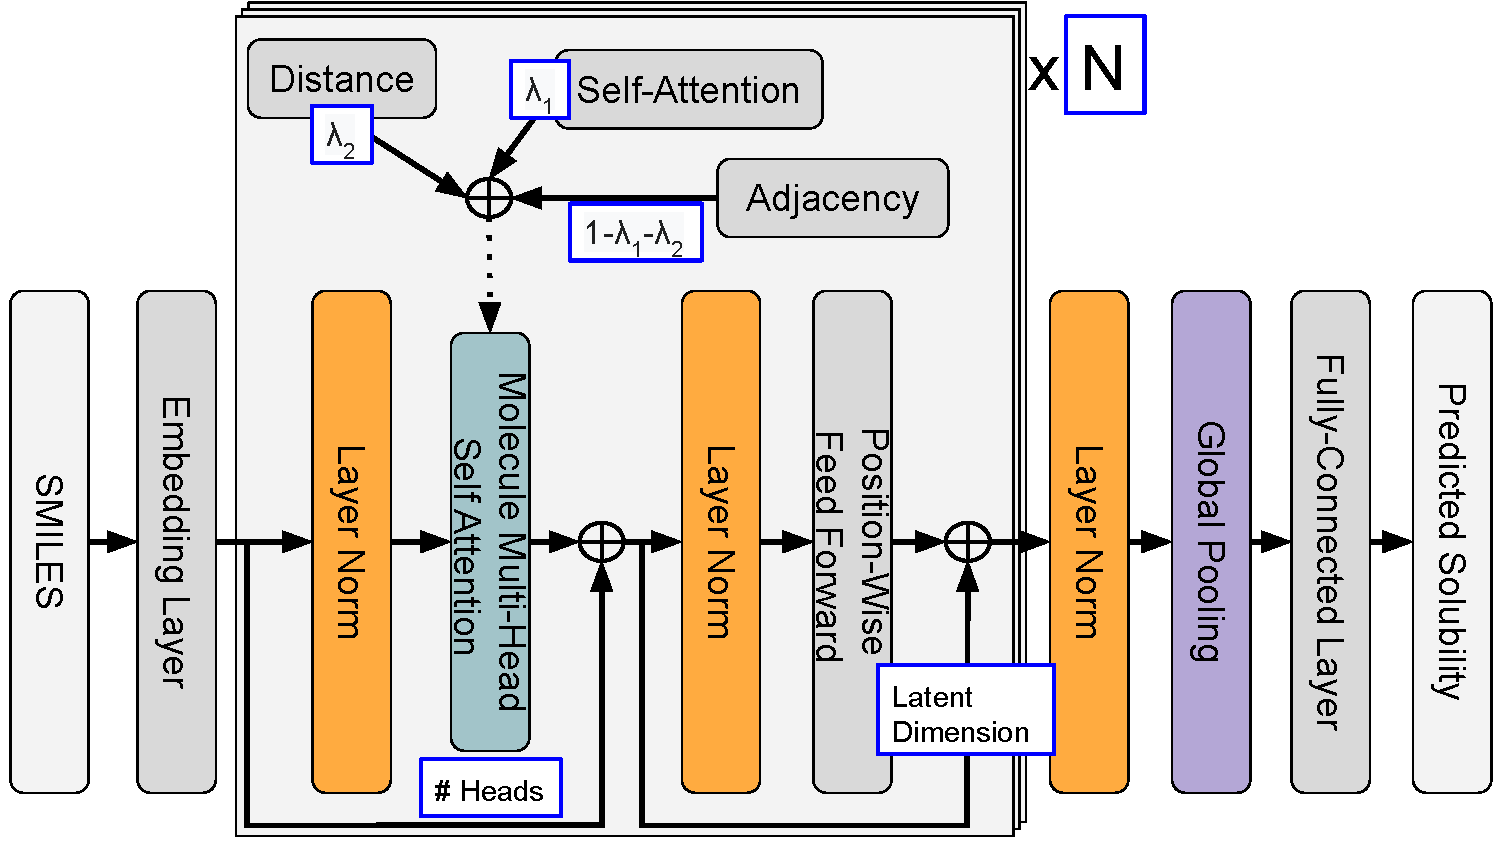
\includegraphics[width=\linewidth]{figures/soltrannet_architecture.pdf}
    \caption{General Architecture of SolTranNet. Each item in a blue box is a tuned hyperparameter, whose values were tested as shown in Figure~\ref{tab:archsweep}.}
    \label{fig:architecture}
\end{figure}

\begin{figure}[tb]
    \subfloat[Optimizer Hyperband Sweep]{
        \centering
        \begin{tabular}{|c|c|}
        \hline
            Parameter & Range \\
        \hline
            Training Epochs & [250, 2000]  \\
            Loss Function & MSE, MAE, Huber  \\
            Learning Rate & [0.0001, 0.1]  \\
            Momentum & [0.5, 0.9]  \\
            Optimizer & SGD, Adam  \\
            Weight Decay & [0, 0.5]  \\
            Dimension of Conformer Generation & 2D, 3D  \\
            Scaffold CCV fold & 0 \\
            Target & minimize test RMSE  \\
        \hline
        \end{tabular}
        \label{tab:initsweep}
    }
    
    \subfloat[Architecture Grid Search]{
        \centering
        \begin{tabular}{|c|c|}
        \hline
            Parameter & Range \\
        \hline
             Dimension of Conformer Generation & 2D, 3D  \\
             Latent Dimension of Encoder & 2, 4, \textbf{8}, 16, 32, 64, 128, 256, 512, 1024  \\
             Dropout & 0, \textbf{0.1}  \\
             Number of Attention Heads (\#Heads) & \textbf{2}, 4, 8, 16, 32  \\
             $\lambda_1$ Attention & 0.25, 0.33, \textbf{0.5}  \\
             $\lambda_2$ Distance & \textbf{0}, 0.33  \\
             Number of Encoder Stacks (\#Stacks) & 2, 4, 6, \textbf{8}, 16  \\
             Scaffold CCV folds & 0, 1, 2  \\
             Loss Function & Huber  \\
             Learning Rate & 0.04  \\
             Momentum & 0.06  \\
             Optimizer & SGD  \\
             Weight Decay & 0  \\
         \hline
        \end{tabular}
        \label{tab:archsweep}
    }
    \caption{Two stage hyperparameter sweep for SolTranNet. The Optimizer sweep was performed via using Weights and Bias's hyperband sweeping tool, with the target to minimize the test set RMSE. The Architecture sweep was a grid search over the listed parameters after the optimizer hyperparameters were set from the first stage. The deployed version of SolTranNet uses the hyperparameters in bold.}
    \label{tab:wandsweep}
\end{figure}

In order to select the best performing model, we calculated the $R^2$ and the root mean square error (RMSE) of the predicted solubility.
Since the solubility values in AqSolDB and other solubility datasets span several orders of magnitude, the $R^2$ correlation metric is easier to perform well on.
Thus, we selected our best performing model by its RMSE performance on our independent test set.
Additionally, as we intend for this tool to be deployed for use on potentially very large datasets, we took into account the speed of SolTranNet in evaluating the results of our hyperparameter search. 

\subsection{Final model training}
The final architecture of SolTranNet utilized the following hyperparameters: 0.1 dropout, 0 lambda distance, 0.5 lambda attention, 2 attention heads, a hidden dimension of size 8, and 8 stacks in the transformer encoding layer. A 2D molecular representation was selected because it provided statistically equivalent results to 3D representations (Figure~\ref{fig:2dv3drmse}) without the computational burden of generating a 3D conformation or computing a distance matrix.
The molecular embedding layer was unchanged from the initial MAT implementation\cite{MAT} where each atom is represented as a node with a feature vector as shown in Fig~\ref{tab:atomembed}.
In order to select the final deployed model, we trained 5 models with different random seeds on all of the data in AqSolDB utilizing the Huber loss function, the SGD optimizer with momentum of 0.06, no weight decay, and a learning rate of 0.04.
We dynamically stopped training after performance on the training set stopped improving for 8 epochs.
After training stopped, we selected the model architecture with the best average RMSE performance on our independent test set and selected the best performing model from within that architecture class (Fig~\ref{fig:dynsweep}).

%%%%%%%%%%%%%%%%%%%%%%%%%%%%%%%%%%%%%%%%%%%%%%%%%%%%%%%%%%%%%%%%%%%%%
%% Results
%%%%%%%%%%%%%%%%%%%%%%%%%%%%%%%%%%%%%%%%%%%%%%%%%%%%%%%%%%%%%%%%%%%%%
\section{Results}

We first show a sampling of results of the hyperparameter sweep that resulted in the final model selection.
We then show the speed benefit of using 2D conformers to process the SMILES string input without a loss of prediction performance.
We also analyze the effect of rare atom types on the efficacy of SolTranNet.
Lastly, we compare SolTranNet to a variety of other published ML-based solubility models.

\subsection{Selecting the Final Architecture}

In order to determine the final architecture of SolTranNet, we performed the two stage hyperparameter search as described in Methods.
Table~\ref{tab:solsearchrmse} shows the RMSE performance of several models from the search on the 3 fold scaffold split of AqSolDB.
The models shown we selected as the top RMSE performers of each class of models, where the class is determined by the number of parameters for said model.
Note that for each combination of hyperparameters, only a single model was evaluated.
Contrary to expectation, we find that models with fewer parameters tended to perform better at solubility prediction for this dataset.
This was mainly driven by better performance on Fold1, which is the most challenging split due to the distribution of solubilities in the test set being markedly different from the training set as shown in Fig~\ref{fig:solhists}.
We mainly focus on the RMSE metric, as since the large range of true predicted values makes it easier to achieve a higher Pearson $R^2$.
The Pearson $R^2$ was also calculated, and is provided in Table~\ref{tab:solsearchr2}.

\begin{table}
    %\centering
    \begin{tabular}{|c|c|c|c|c|c|c|}
        \hline
         Model & Parameters & CCV RMSE & Fold0 RMSE & Fold1 RMSE & Fold2 RMSE & Ind RMSE \\
         \hline
         MAT & 42,049,537 & 2.007 & 1.231 & 3.075 & 1.058 & 2.113  \\
         \hline
         0 & 21,061,633 & 1.449 & 1.161 & 1.959 & 1.054 & 1.914 \\
         1 & 502,529 & 1.467 & 1.231 & 1.972 & 1.028 & 1.946 \\
         2 & 336,385 & 1.377 & 1.260 & 1.682 & 1.126 & 1.870 \\
         3 & 336,385 & 1.454 & 1.239 & 1.857 & 1.165 & 1.949 \\
         4 & 22,657 & 1.297 & 1.187 & \textbf{1.582} & 1.066 & 1.903 \\
         5 & 11,905 & \textbf{1.271} & \textbf{1.130} & 1.605 & \textbf{0.998} & 1.923 \\
         6 & 11,905 & 1.350 & 1.272 & 1.680 & 1.012 & 1.903\\ \hline \hline
         7 & 3,393 & 1.459 & 1.172 & 1.916 & 1.159 & \textbf{1.779}\\ \hline \hline
         8 & 2,609 & 1.376 & 1.169 & 1.788 & 1.055  & 1.973 \\
         9 & 2,609 & 1.454 & 1.252 & 1.919 & 1.043  & 1.973 \\
         \hline \hline
         Elastic & 1,463 & 1.835 & 1.843 & 1.965 & 1.687  & 2.090\\
         Lasso & 1,077 & 1.876 & 1.914 & 1.984 & 1.719 & 2.136\\
         PLS & 2,048 & 2.413 & 3.085 & 2.082 & 1.902 & 2.081\\
         Ridge & 2,048 & 2.239 & 2.503 & 2.032 & 2.155 & 2.312 \\
         \hline
    \end{tabular}
    \caption{SolTranNet model hyperparameter search for predicting solubility RMSE on the scaffold-based clustered cross-validation splits of AqSolDB (CCV) and our independent test set (Ind). Additionally, all models outperform linear approaches trained on RDKit fingerprints using scikit-learn\cite{scikit-learn}. The isolated row (model 7) is the final SolTranNet architecture.}
    \label{tab:solsearchrmse}
\end{table}

We then quantified SolTranNet's generalization by training 5 different models on the entirety of AqSolDB and testing them on our withheld independent set as shown in Table~\ref{tab:deployed}.
Notably, an ensemble of 5 models outperforms the mean of said models, but fails to beat the best performing seed (Figure~\ref{fig:dynsweep}).
As we desire SolTranNet to be as fast as possible, we have elected to deploy a single model with the best performing seed.

\begin{table}
    \begin{tabular}{|c|c|c|c|c|}
        \hline
        Model & Train RMSE & Test RMSE & Train $R^2$ & Test $R^2$ \\
        \hline
        Average of 5 Seeds & 1.171 (0.0504) & 1.878 (0.0925)  & 0.784 (0.00643) & 0.509 (0.0445)\\
        Ensemble & \textbf{1.068} & 1.814 & \textbf{0.798} & 0.517\\
        Deployed & 1.144 & \textbf{1.711} & 0.777 & \textbf{0.577}\\
        \hline
    \end{tabular}
    \caption{Performance of 5 different seeds of SolTranNet. Each model was trained on all of AqSolDB and tested on our independent test set. We note that the ensemble outperforms each model on average, but fails to beat the best performing seed. Deployed refers to the single best performing model.}
    \label{tab:deployed}
\end{table}

\subsection{Conformer Generation}

The first part of the SolTranNet pipeline is to create the molecular graph representation of each input molecule's SMILE string.
Part of this representation is the calculation of the distance matrix, which stores how far apart each atom is from every other atom.
In the MAT implementation this matrix is calculated by using RDkit to generate a 3D conformer for the molecule, which can be a potentially costly process.
Thus, as shown in Figure~\ref{fig:2dv3drmse} and Figure~\ref{fig:2dv3dr2}, we show that using a 2D or 3D conformer does not have a statistically significant difference on RMSE or $R^2$ for the first 10 hyper-parameter combinations of SolTranNet during the architecture sweep ($p=0.144$).
As such, we did not train 3D versions of the models for the remainder of the sweep and instead used distances determined from the 2D representation of the molecule. 
As the final model does not use distance information ($\lambda_2 = 0$), this matrix is not calculated, further accelerating predictions.

\begin{figure}[tb]
    \centering
    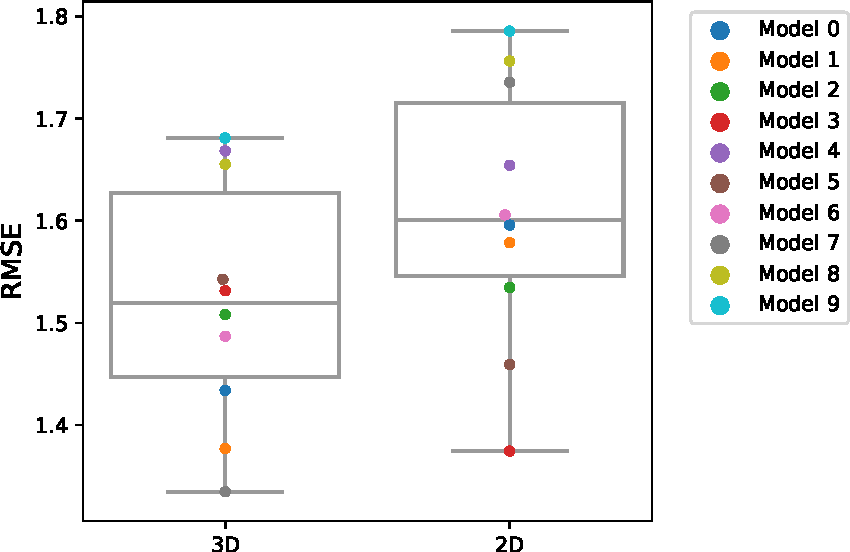
\includegraphics[width=\linewidth]{figures/2dv3d_rmse.pdf}
    \caption{The first 10 models of the SolTranNet architecture sweep RMSE performance dependent on if the distance matrix used 3D conformers of the molecules. There is no statistically significant difference between these two collections ($p=0.144$), however the mean performance is better for the 3D models (1.522 vs 1.608).}
    \label{fig:2dv3drmse}
\end{figure}

\subsection{Salts and Rare Atom Types}
In AqSolDB, salts are explicitly represented and consist of about 11.0\% of the available data.
In addition, due to the atom typing schema of SolTranNet, 9.87\% of the AqSolDB molecules contain atoms that are typed as ``Other,'' i.e. not B, N, C, O, F, P, S, Cl, Br, or I.
These two groups overlap by 75.2\% and 83.9\% respectively; that is, unusual atom types are typically due to the inclusion of salts.
As such, we investigate the effect of fragmenting the salts (only keeping the largest component) and removing successively larger molecules with ``Other" typed atoms from the training data in Figure~\ref{fig:saltfragrmse} and Figure~\ref{fig:saltfragr2}.
Notably, for all comparisons between identical test sets, there is no statistically significant difference between training on the full salt or the fragmented salt for the RMSE evaluations.
We do note that when removing all molecules containing any ``Other'' typed molecule, training on fragmented salts performed better for the $R^2$ evaluation when testing with fragmented salts while having the same performance on testing with normal salts (Figure~\ref{fig:noothersdf2}).
Thus, we elect to train on the full salt, as it allows for less data preprocessing by the user.
Also, as we remove more ``Other" typed molecules from the training and testing data, we observe a performance increase, as expected.
Since these ``Other" typed atoms are potentially encountered in a drug discovery setting, we elected to keep them in SolTranNet's training set, but have molecules with such types raise a warning to the user.

\begin{figure}[tb]
    \centering
    \begin{subfigure}[t]{0.48\textwidth}
        \centering
        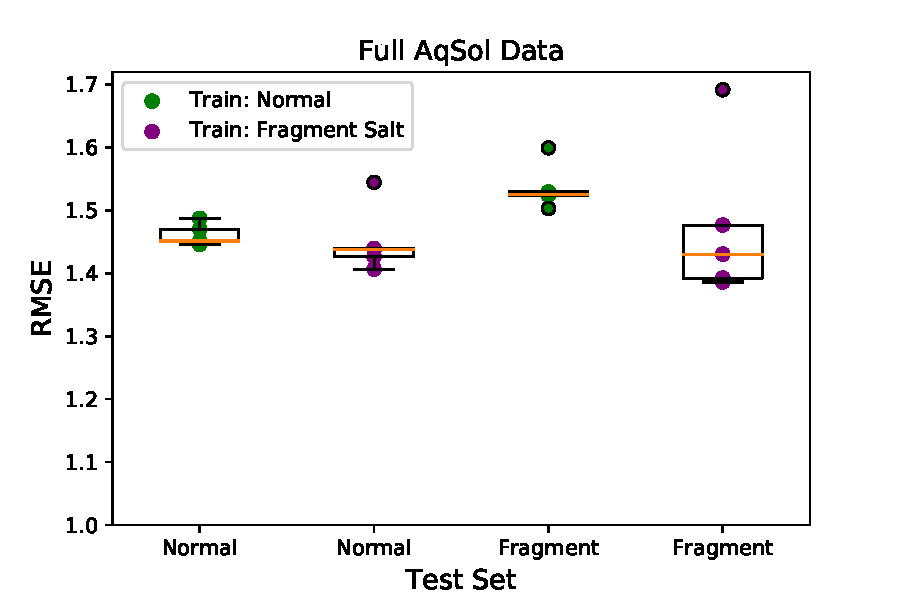
\includegraphics[width=\linewidth]{figures/full_saltfragfirst_RMSEs_boxplots.pdf}
    \end{subfigure}%
    \hfill
    \begin{subfigure}[t]{0.48\textwidth}
        \centering
        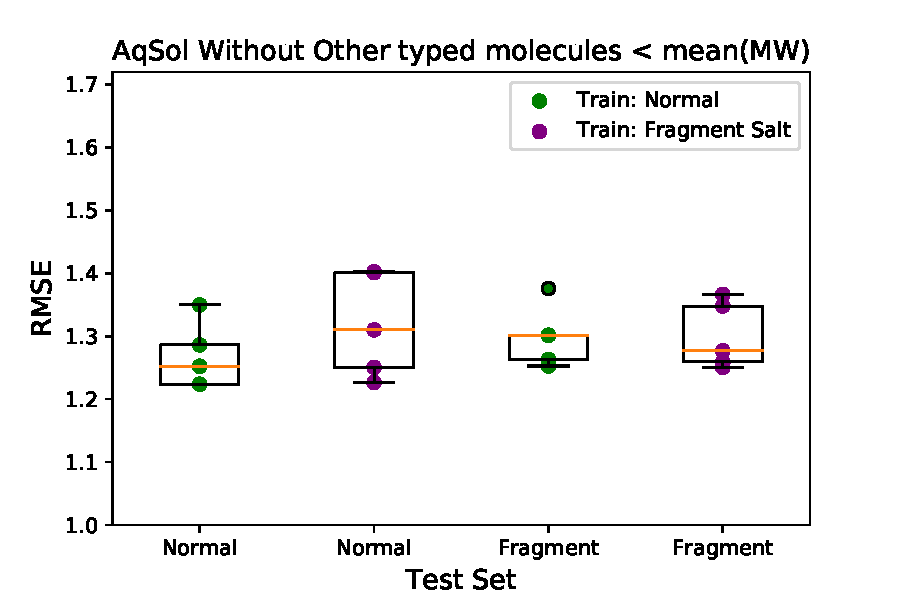
\includegraphics[width=\linewidth]{figures/othersMW_saltfragfirst_RMSEs_boxplots.pdf}
    \end{subfigure}
    
    \begin{subfigure}[t]{0.48\textwidth}
        \centering
        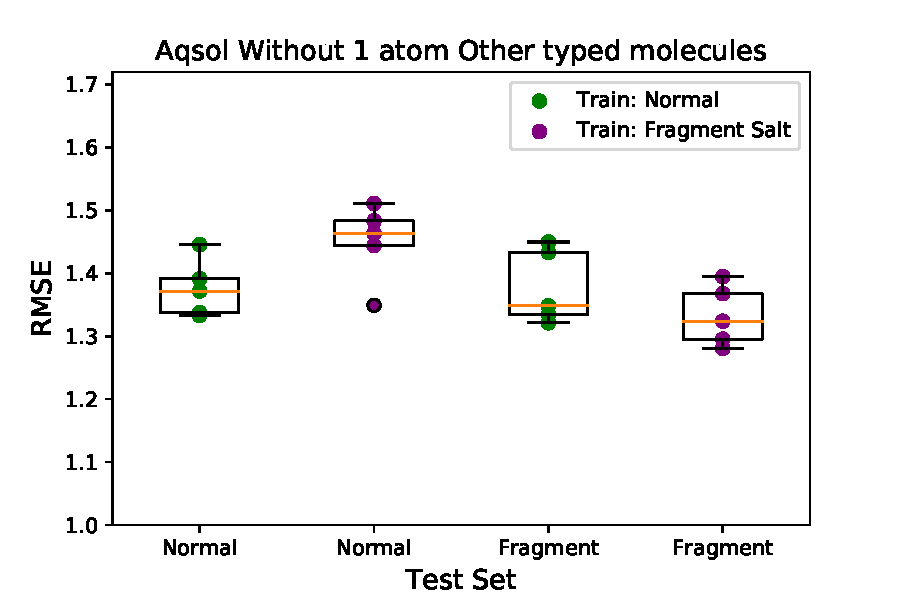
\includegraphics[width=\linewidth]{figures/others2plus_saltfragfirst_RMSEs_boxplots.pdf}
    \end{subfigure}%
    \hfill
    \begin{subfigure}[t]{0.48\textwidth}
        \centering
        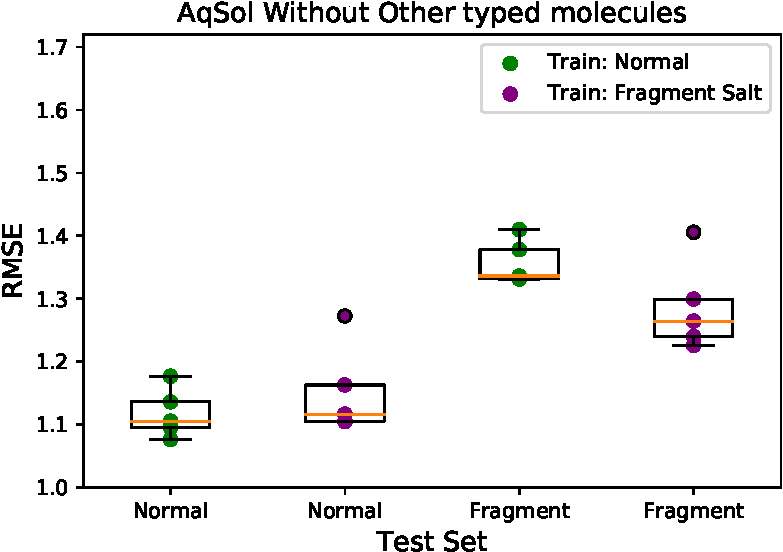
\includegraphics[width=\linewidth]{figures/noothers_saltfragfirst_RMSEs_boxplots.pdf}
    \end{subfigure}
    \caption{RMSE of 5 different SolTranNet trained on the scaffold split of AqSolDB. The horizontal axis is dependent on if the salts were fragmented in the test set, while the colors of the boxplot are dependent on if the salts were fragmented in the training set. Each plot has successively fewer data points in the training and testing sets by more stringently removing atoms which would be embedded as ``Other type'' during training. There is no statistically significant difference in performance on the test set between training on Normal, or Fragmented Salts for all sets.}
    \label{fig:saltfragrmse}
\end{figure}

\subsection{Run-time Performance}

Lastly, we seek to benchmark the run-time performance of SolTranNet.
For benchmarking, we determined the mean time it takes to go from a SMILES string to a solubility prediction for the 132 molecules provided by SC2, with a batch size of 32.
Table~\ref{tab:timings} shows the mean and standard deviation of 10 runs performed on a machine with an Nvidia Titan-XP graphics card, and using 1 core of an Intel(R) Core(TM) i7-4930K CPU.
Notably for the original MAT implementation, utilizing the 3D conformer generation takes 36 times longer when utilizing the GPU (only 4 times longer on CPU).
SolTranNet, with its fewer number of parameters and skipping of the conformer generation process, runs 1.6 times faster on the GPU (9.7 times faster on CPU) than MAT utilizing the 2D conformer generation.
With our 2D implementation and running on a single GPU 1 million molecules can be predicted in about 36 minutes (51 minutes on CPU).

%This is for the version that is still calculating the distance matrix, even though it all gets 0'd out.
%I'm working on adding a row for the deployed version which skips this calculation entirely
%It's still being coded, and then we need to train it and verify performance.

\begin{table}
    %\centering
    \begin{tabular}{|c|c|c|}
        \hline
         Model & Time (s/mol) GPU & CPU \\
         \hline
         MAT 3D & 0.1233 (0.001928) & 0.1493 (0.002315) \\
         MAT 2D & 0.003472 (0.00015) & 0.02968 (0.002516) \\
         STN & 0.002132 (0.000018) & 0.0030451 (0.000058)\\
         \hline
    \end{tabular}
    \caption{Mean time for the model to predict a solubility from a SMILES string for the original MAT implementation and SolTranNet (STN). The predictions were for the molecules in the Solubility Challenge 2 dataset. We report the mean and standard deviation (in parenthesis) for each model utilizing 10 runs in seconds per molecule. All predictions were performed on a machine with a Nvidia Titan-XP graphics card, and an Intel(R) Core(TM) i7-4930K CPU, with a batch size of 32.}
    \label{tab:timings}
\end{table}


\subsection{SolTranNet Performance on Other Datasets}

In order to compare SolTranNet to other methods, we evaluated SolTranNet on four recently published solubility training and testing sets, as shown in Table~\ref{tab:othersetsrmse} and Table~\ref{tab:othersetsr2}.
To provide fair comparisons, we evaluate both models trained with the provided training and testing data and the deployed version of SolTranNet, which is trained on AqSolDB.
For each paper we initially trained five models with the same dynamic stopping criteria as our training set.
However, for the dataset provided by \citet{lovric} and \citet{boobier}, this performed very poorly and stopped training early, due to the much smaller size of the training sets (530 and 75 molecules respectively) as compared to our AqSolDB training sets (6655 CCV and 9982 full).
As such, we trained new models for 1000 and 500 epochs respectively for those sets.
For the datasets provided by \citet{cui}, \citet{lovric}, and \citet{boobier}, SolTranNet's best performing model trained on the provided datasets achieves similar results to the method reported in the respective paper.
However, for the Second Solubility Challenge data\cite{llinas}, SolTranNet has much worse performance than the top submitted method and ranks in the lower quarter of the submitted methods.

\begin{table}
    \centering
    \begin{tabular}{|c|c|c|c|c|c|}
        \hline
        Dataset &  Reported & STN Training &  STN Best & STN Deployed & Overlap \\
        \hline
        Cui2020 & 0.681 & 0.860(0.215) & 0.624 & 0.813 & 0/62 \\
        Boobier2017 & 0.985 & 1.274(0.178) & 1.010 & 0.845 & 23/25 \\
        Lovric2020 & 0.720 & 0.898(0.101) & 0.720 & 0.854(0.0672) & 151.4/166 \\
        Llinas2020 set1 & 0.780 & 1.119(0.163) & 0.952 & 1.004 & 79/100 \\
        Llinas2020 set2 & 1.060 & 1.811(0.328) & 1.243 & 1.295 & 18/32 \\
        \hline
    \end{tabular}
    \caption{RMSE performance of SolTranNet (STN) on other published datasets. For SolTranNet Training, we trained five different seeds of our final architecture on the provided training and testing splits and report the mean and standard deviation (in parentheses). The SolTranNet Deployed column is using our final deployed model to predict the provided test set. The final column is the overlap of the provided test set with our deployed model's training set. Notably the Lovric set had five different randomly selected splits for training and testing, which is why there is a mean in the Deployed and Overlap columns.}
    \label{tab:othersetsrmse}
\end{table}

This prompted us to analyze how useful SolTranNet is compared to these other models at classification of soluble compounds, which is a typical use case for such a model in a virtual screening pipeline.
To refactor the problem as a classification task, we define a soluble compound as a compound with $logS > -4$ and an insoluble compound as having $logS \leq -6$.
These bounds were selected as a molecule having $logS \leq -6$ this would correspond to being unable to obtain a micromolar solution of the drug, and a $logS > -4$ corresponds to being able to obtain a 100 micromolar solution of the drug.
For this analysis molecules with $-6 < logS <= -4$ were discarded.
This process resulted in 74 out of 132 initial molecules in the SC2 dataset being retained for analysis.
We then calculated the sensitivity and false discovery rate of SolTranNet and each method submitted to the SC2 competition, as shown in Figure~\ref{fig:sc2redo}.
With these definitions SolTranNet has a sensitivity of 94.8\% and a false discovery rate of 1.30\%, which had it tied for fourth place and second place respectively.

\begin{figure}[tb]
    \centering
    \begin{subfigure}[t]{0.48\textwidth}
        \centering
        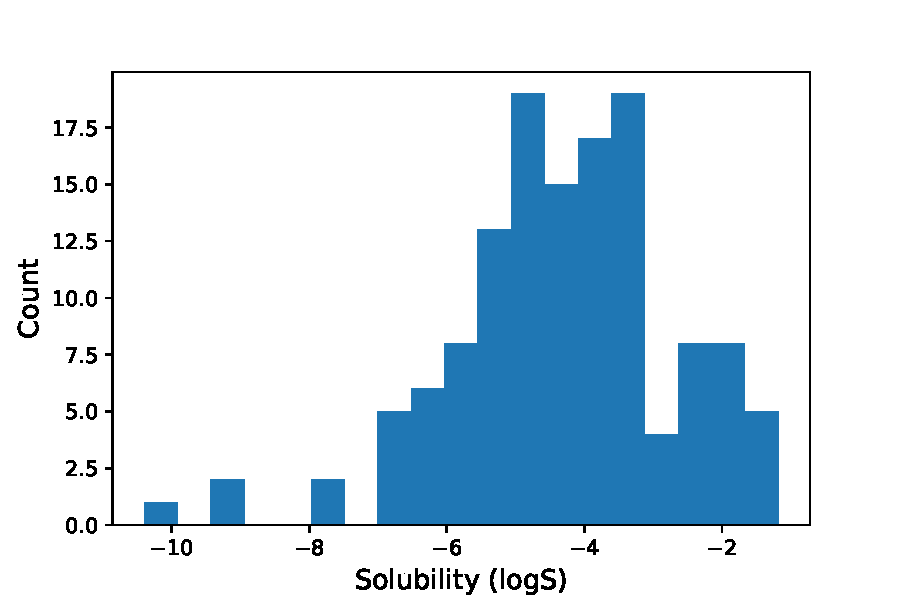
\includegraphics[width=\linewidth]{figures/histogram_solchal2_true_logs.pdf}
        \caption{Distribution of solubility values in the Solubility Challenge 2 test sets, with bin width of 0.5.}
    \end{subfigure}
    
    \begin{subfigure}[t]{0.48\textwidth}
        \centering
        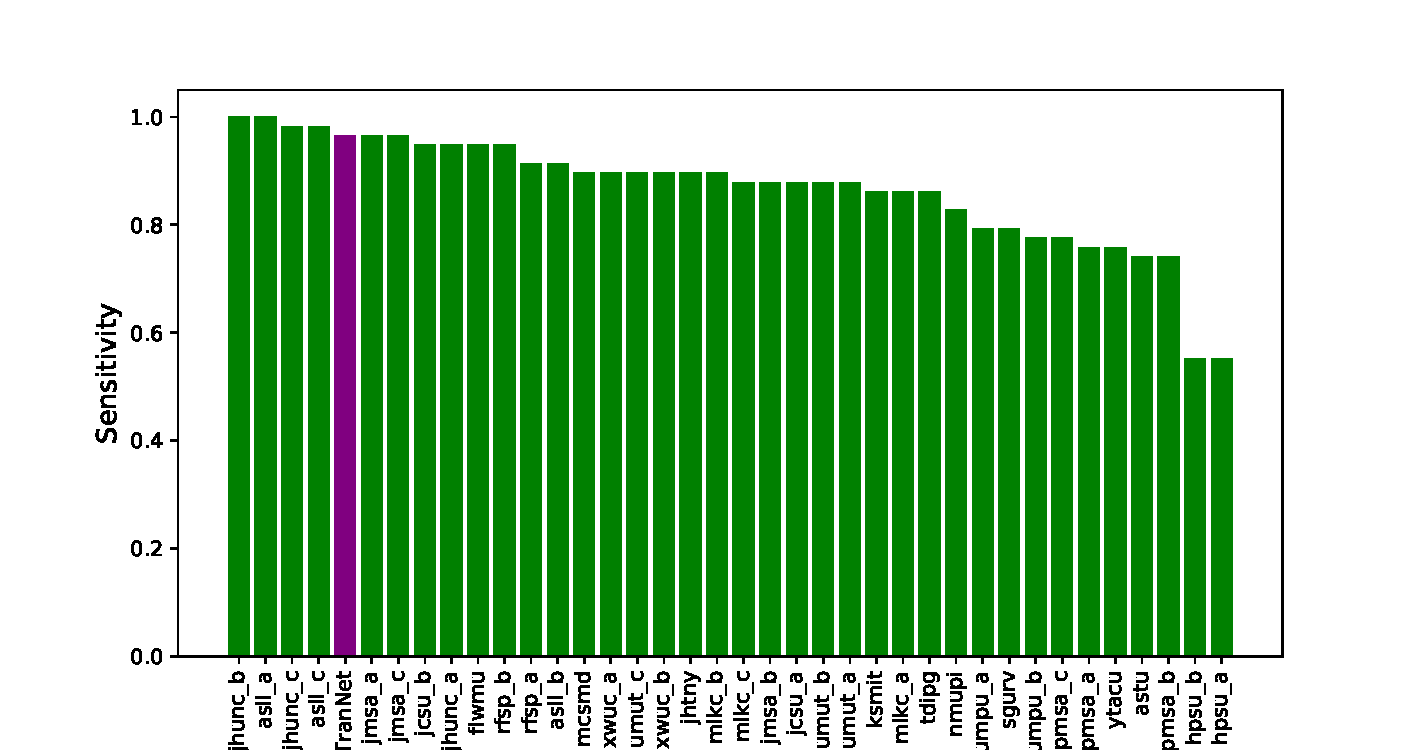
\includegraphics[width=\linewidth]{figures/hit_solchal2.pdf}
        \caption{Sensitivity of submitted predictions on the Solubility Challenge 2 test sets. SolTranNet is shown in purple.}
    \end{subfigure}%
    \hfill
    \begin{subfigure}[t]{0.48\textwidth}
        \centering
        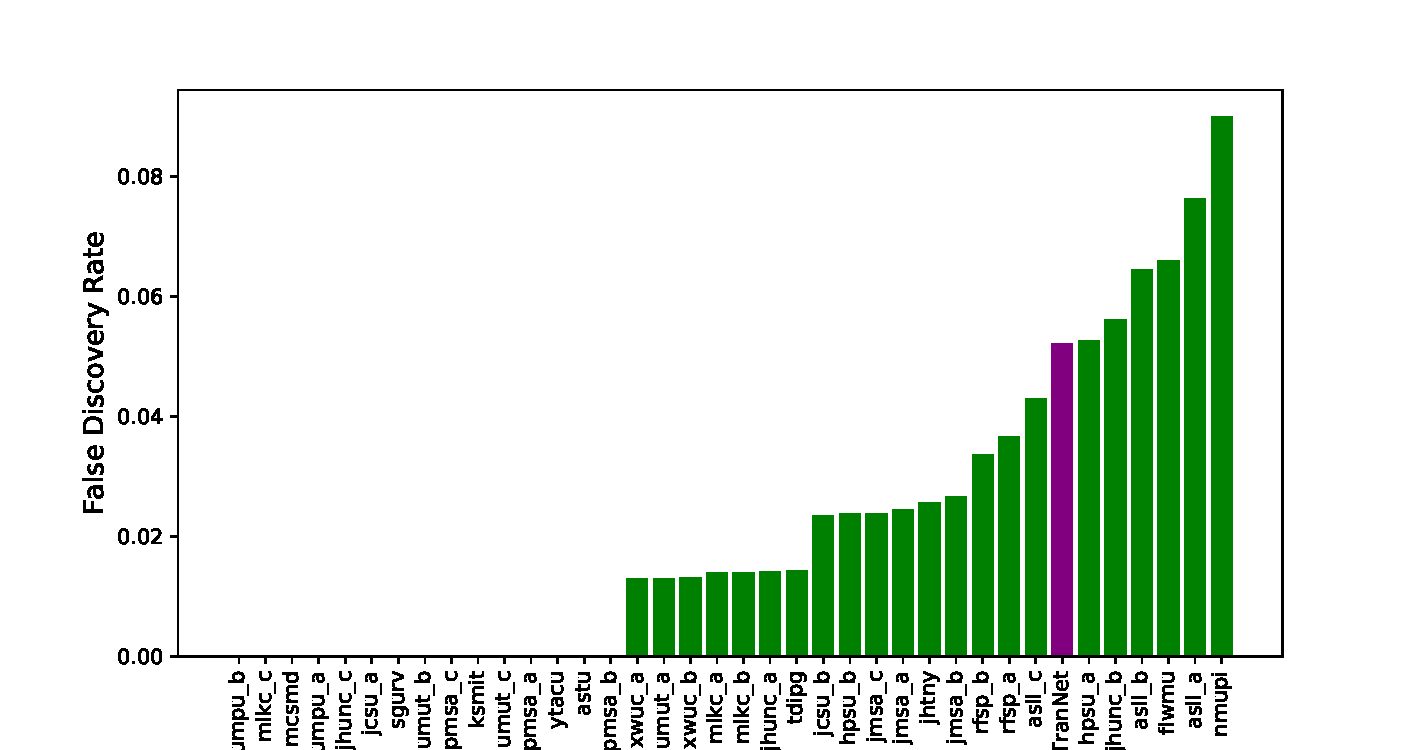
\includegraphics[width=\linewidth]{figures/fail_solchal2.pdf}
        \caption{False discovery rate of submitted predictions on the Solubility Challenge 2 test sets. SolTranNet is shown in purple.}
    \end{subfigure}
    \caption{Recontextualizing the Solubility Challenge 2 data, as if we submitted SolTranNet. (a) Distribution of both test sets provided for the challenge where each bin is 0.5 units wide. We turned the predictions into a classification of solubility, where a molecule is soluble if its logS $> -4$, and insoluble if its logS $\leq -6$. We then calculated the sensitivity (b) and false discovery rates (c) of each contestant in Solubility Challenge 2 and SolTranNet. SolTranNet performs near state of the art in terms of sensitivity (94.8\%) and false discovery rate (1.30\%) with these definitions.}
    \label{fig:sc2redo}
\end{figure}

%%%%%%%%%%%%%%%%%%%%%%%%%%%%%%%%%%%%%%%%%%%%%%%%%%%%%%%%%%%%%%%%%%%%%
%% Discussion
%%%%%%%%%%%%%%%%%%%%%%%%%%%%%%%%%%%%%%%%%%%%%%%%%%%%%%%%%%%%%%%%%%%%%
\section{Discussion}

We described SolTranNet, a molecule attention transformer for predicting aqueous solubility, and evaluated it on a variety of datasets.
During model optimization we show that SolTranNet outperforms linear ML approaches (Table~\ref{tab:solsearchrmse}), and obtains competitive performance to other ML methods at aqueous solubility (Table~\ref{tab:othersetsrmse} and Fig~\ref{fig:sc2redo}).
Of particular note, during our hyperparameter sweep (Table~\ref{tab:solsearchrmse}) we observed that smaller ML models perform better than their larger counterparts.
This goes contrary to the observations of \citet{cui} who observed that deeper models performed better.
Yet SolTranNet's best performing model when given the same training and testing data achieved better performance than the 20-layer ResNet architecture utilized by \citet{cui} (Table~\ref{tab:othersetsrmse}).
We suspect that the small size of the available training data is the reason that larger models perform worse.

The available solubility data is quite small, with ``large datasets'' being composed of thousands of data points.
Small training set sizes make it easier for ML methods to overfit their training data, and limits their ability to generalize.
We observed such a phenomenon, especially with our larger models, during our hyperparameter sweep (Table~\ref{tab:solsearchrmse}).
We hypothesize that the smaller models, with less of an ability to overfit to their training data, are more suited to solubility prediction until more training data becomes available.
Data augmentation is a potential approach to expand the available data, but we leave this to future work.

Another concern with the available solubility data is the small size of the testing sets used in the community.
With test sets in the tens or low hundreds of molecules, there is a limit on the power of the conclusions that we can draw from model performance on them.
Even with training sets of several thousand molecules, we observe markedly worse performance (Fold1 column of Table\ref{tab:solsearchrmse}) when test set distributions are substantially different from the training set (Figure~\ref{fig:solhists}).
This indicates that our models may not be learning a set of completely generalizable molecular features to make their predictions.
The large range of the possible values in AqSolDB (14 log units) makes it easier to achieve high correlation statistics, which is why we favored analysis of the RMSE of the given predictions to compare model performance.

Notably, SolTranNet had markedly worse performance on the Solubility Challenge 2 dataset than the best performing group (Table~\ref{tab:othersetsrmse}).
However, it should also be noted that the test sets for the Solubility Challenge 2 were not blind.
This indicates that the most relevant comparison to the reported metrics is the STN Best model in Table~\ref{tab:othersetsrmse}, as it is selected with knowledge of performance on the test set.
SolTranNet also exhibited the largest amount of training variability on these test sets (with the best model having a 0.2 and 0.6 RMSE performance boost respectively as compared to the mean), which indicates that we could potentially have a large performance boost by optimizing the SolTranNet architecture with this test set in mind.

Even the best reported models have an RMSE of over half a log unit, which raises the question of what level of performance makes a model useful for a drug discovery pipeline.
In order to investigate this, we restructured the evaluation into a classification task, as described in SolTranNet Architecture on Other Datasets section.
We then chose the sensitivity and false discovery rate as our metrics of interest, as we desire a model that correctly identifies soluble compounds (high sensitivity) and avoids falsely identifying insoluble compounds (low false discovery rate).
SolTranNet achieves this goal with a sensitivity of 94.8\% and a false discovery rate of 1.30\%, which is comparable to the other methods submitted to this competition.

We have shown that SolTranNet, through its molecule attention transformer architecture, is amenable to predicting aqueous solubility from the SMILES string of a molecule, and outperforms linear ML approaches.
During our hyperparameter optimization in Table~\ref{tab:solsearchrmse} and Table~\ref{tab:solsearchr2}, we demonstrate that models with more parameters do not perform better in our scaffold-based CCV splits and also exhibit worse performance on an independent test set.
The smaller size of SolTranNet and not needing to calculate a distance matrix makes it run 58 times faster than the original MAT implementation (Table:\ref{tab:timings}).
SolTranNet performs comparably well to other current ML based models, as shown in Table~\ref{tab:othersetsrmse},\ref{tab:othersetsr2} and Figure~\ref{fig:sc2redo}.
We have deployed SolTranNet as a \textsc{pip} installable package for easy integration into drug discovery pipelines, and its source code is available at \url{https://github.com/gnina/SolTranNet}.

%%%%%%%%%%%%%%%%%%%%%%%%%%%%%%%%%%%%%%%%%%%%%%%%%%%%%%%%%%%%%%%%%%%%%
%% The "Acknowledgement" section can be given in all manuscript
%% classes.  This should be given within the "acknowledgement"
%% environment, which will make the correct section or running title.
%%%%%%%%%%%%%%%%%%%%%%%%%%%%%%%%%%%%%%%%%%%%%%%%%%%%%%%%%%%%%%%%%%%%%
\begin{acknowledgement}


The authors thank Andrew McNutt and Jonathan King for their insightful contributions during the preparation of this manuscript.

This work is supported by R01GM108340 from the National Institute of General Medical Sciences, and by a GPU donation from the NVIDIA corporation.

\end{acknowledgement}

%%%%%%%%%%%%%%%%%%%%%%%%%%%%%%%%%%%%%%%%%%%%%%%%%%%%%%%%%%%%%%%%%%%%%
%% The same is true for Supporting Information, which should use the
%% suppinfo environment.
%%%%%%%%%%%%%%%%%%%%%%%%%%%%%%%%%%%%%%%%%%%%%%%%%%%%%%%%%%%%%%%%%%%%%
\begin{suppinfo}

%This will usually read something like: ``Experimental procedures and
%characterization data for all new compounds. The class will
%automatically add a sentence pointing to the information on-line:
Supporting Information Available: Supplementary Figures~\ref{fig:dynsweep}-\ref{fig:saltfragr2} and Tables~\ref{tab:solsearchr2}-\ref{tab:othersetsr2}.
\end{suppinfo}

%%%%%%%%%%%%%%%%%%%%%%%%%%%%%%%%%%%%%%%%%%%%%%%%%%%%%%%%%%%%%%%%%%%%%
%% The appropriate \bibliography command should be placed here.
%% Notice that the class file automatically sets \bibliographystyle
%% and also names the section correctly.
%%%%%%%%%%%%%%%%%%%%%%%%%%%%%%%%%%%%%%%%%%%%%%%%%%%%%%%%%%%%%%%%%%%%%
\bibliography{references}
\end{document}